\documentclass{IEEEtran}
\usepackage{tikz}
\tikzstyle{box}=[rectangle,draw=black, ultra thick, minimum size=1cm]
\usepackage{algorithm}
\usepackage{algpseudocode}
\usepackage{graphicx}
\usepackage{caption}
\usepackage{listings}
\usepackage{caption}
\usepackage{lipsum}
\usepackage{amsmath}
\usepackage[hidelinks]{hyperref}

\author{Alp Gokcek \\gokcekal@mef.edu.tr \\ MEF University \\ \today}
\title{\href{https://github.com/alpgokcek/turkey-navigation-ai}{Navigation on Turkey Map}}

\renewcommand\IEEEkeywordsname{Keywords}


\begin{document}
	\maketitle
	\begin{abstract}
		Search problem is a well-known issue in the field of Artificial Intelligence. There are various algorithms designed for this problem, such as Dijkstra, A-star, Breadth-First Search, and much more. This paper has demonstrated and applied one of the most efficient search algorithms for the problem, which is the A-star algorithm for finding the shortest path on a given map. 
	\end{abstract}
\begin{IEEEkeywords}
	Shortest-path, A-star search, search algorithms.
\end{IEEEkeywords}
\section{Introduction \& Problem Statement\label{introduction}}
Searching is a comprehensive technique of problem-solving in AI. Before evaluating the problem, there are several terminological words and phrases that have to be known. 
\subsection{Terminology}
There are several terminological things to know during the paper. These are:
\begin{itemize}
	\item \textbf{Node(State):} All potential outcomes of the problem with a unique identification
	\item \textbf{Transition:} Traveling between states or nodes.
	\item \textbf{Starting Node:}  Where to start searching
	\item \textbf{Goal Node:} The target to stop searching.
	\item \textbf{Cost:} Cost for the path from a node to another node. This value can be the distance between nodes, time, and much more..
	\item \textbf{g(n):} This function returns the exact cost of the path from the starting node to any node $n$.
	\item \textbf{h(n):} This function returns heuristic estimated cost from node n to the goal node.
	\item \textbf{f(n):} Lowest cost in the neighboring node n
\end{itemize} \cite{astar-tds}
\subsection{Problem}
These algorithms aim to travel from a starting node to a goal node by transiting through transitional nodes. It is not just used in shortest-path problems but also in single-player games like puzzles, Sudoku, and many more. For instance, in N-puzzle or also known as Sliding Puzzle, there is a square-shaped board, and it has N-tiles with one empty space that is available for sliding a block. In this case, the approach is to find all possible solutions through moving each block one by one until reaching the goal state.\\

In the shortest-path problem, as the name refers, the main goal is to find the shortest path between 2 nodes, in our case these nodes are cities, if any possible path exists. \cite{shortest-path} This problem is also a search problem and a search operation is performed from starting node to the goal node. There are several algorithms designed for solving searching problem and they have different advantages over each other. The most known algorithms can be listed as:\\
\begin{itemize}
	\item Breadth-First Search
	\item Depth-First Search
	\item A-star(A*) Search
	\item Greedy Best First Search
	\item Uniform Cost Search (Dijkstra's Algorithm)
\end{itemize}
The most used ones are A* Search Algorithm, Breadth-First, and the Dijkstra Algorithm. \cite{astar-redblob} Search pattern differences of Breadth-First, Dijkstra and A-star search algorithms is illustrated in Figure \ref{search-patterns}. \\


\includegraphics[scale=1.35]{search.jpg}
\captionof{figure}{Search patterns of Breadth-First, Dijkstra and A* \cite{astar-redblob}\label{search-patterns}\\}

\subsection{A* (A-star) Search Algorithm}
\textit{A* algorithm} is a heuristics-based algorithm for the shortest path-finding. It is the optimized version of the Dijkstra Algorithm for a single target. A* algorithm aims to reach only the goal node in the shortest path possible, whereas, in the Dijkstra Algorithm, all possible paths from all nodes would be found. In other words, the Dijkstra algorithm is finding the path blind by calculating all the paths possible, whereas, in A-star, it senses the shortest path with the help of the heuristic function. So, if the problem is to reach from one node to another, the Dijkstra Algorithm is not optimal. Therefore, the need for the A* algorithm arose. Its working principle is based on heuristics, at each node that expanded, the heuristic function would be executed, and the cost of transition is calculated. \cite{astar-redblob} The pros and cons of the algorithm could be found below.\\
\subsubsection{Advantages}
The A-star algorithm is a better performing algorithm compared to other search algorithms. There are several pros that can be mentioned:
\begin{itemize}
	\item On the worst case, its complexity is $\mathcal{O}(n\log{}n)$. Other popular search algorithms such as Dijkstra Algorithm has the complexity of $\mathcal{O}(n^2)$.
	\item A-star is optimal since there is a significant difference between the number of nodes expanded during the execution.
	\item If the branching factor is finite and each transition has a fixed cost, then the algorithm becomes complete. \cite{astar-brainkart}\\
\end{itemize}
\subsubsection{Disadvantages}
As each algorithm has downsides, A-star has downsides too. Several cons that can be listed are:
\begin{itemize}
	\item A-star algorithm uses a lot of memory.
	\item The execution speed is highly dependent on the heuristic function $h(n)$. The heuristic function must be admissible 
	\item A-star algorithm is not a uniformed algorithm; in other words, it can only target one node in one execution. For instance, if there are $n$ targets on the graph, A-star would be executed $n$ times, which may or may not be the optimal solution.
\end{itemize}

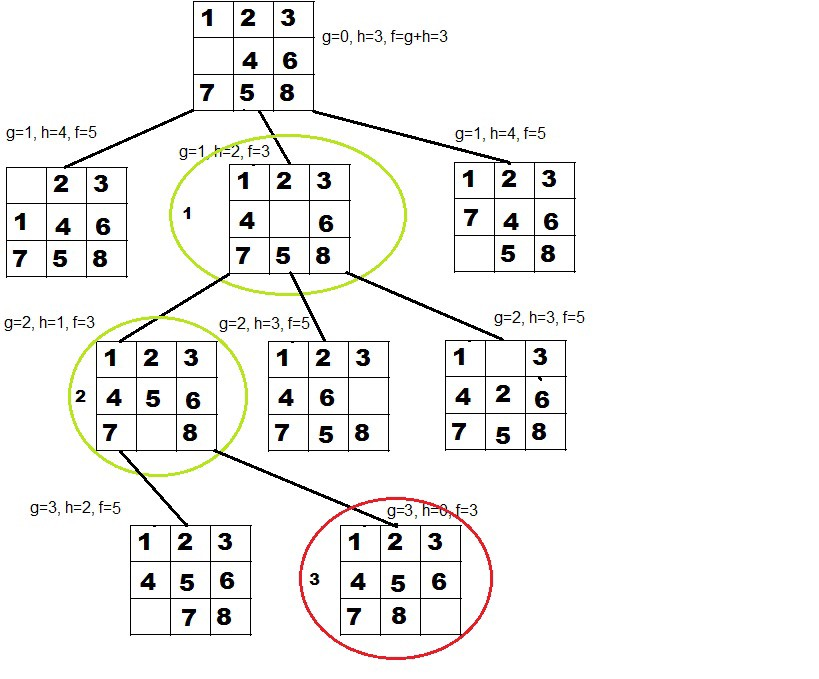
\includegraphics[scale=0.32]{solving-puzzle.jpeg}
\captionof{figure}{Solution for N-puzzle with A* algorithm \label{search-example}\\}

In Figure \ref{search-example}, a sample solution could be found which is solved with A-star algorithm. 

\subsection{Breadth-First Search Algorithm}
Breadth-First search is the intuitive solution for everyone. It is simple compared to other algorithms and it does not consider the costs, thus it explores equally in all directions. This method is significantly useful algorithm but it is not frequently used in shortest-path problems since it is not optimal for this problem at all. 

\subsection{Dijkstra Algorithm}
\textit{Dijkstra's Algorithm} calculates the shortest path from one desired node of the graph to every other node. It is widely used and adopted for many different applications, such as computer networks, road maps, social platforms and much more. There are various implementations of the algorithm; the main difference between them is how they store the vertices of the graph, denoted with $Q$. They can be stored in regular arrays, linked lists, adjacency lists, or tree structures. The algorithm's running time can be represented with the number of edges $|E|$ and the number of vertices $|V|$ using big-o notation. Running time mainly depends on these structures, storing $Q$ in arrays it is $\mathcal{O}(|V|^2)$ but with the help of \textit{min-priority queue} it drops down to $\mathcal{O}((|E| + |V|) \log{|V|})$ time in the worst case. 

\section{Solution Design Process\label{solution-design}}
For this problem, the initial approach was to implement the Dijkstra Shortest Path Algorithm and prompt the outcome to the user after the execution of the algorithm. As mentioned in the previous section, Dijkstra Algorithm is a uniformed algorithm; in other words, algorithm blindly finds the shortest paths from each node to every node. This approach is time consuming and not optimal since our aim is to find just a path between start node to goal node. It is redundant to find paths that will not be used. Thus, there was a need to improve the performance of the program. The second approach was to implement the A-star Search Algorithm. As mentioned in the previous section, the A-star algorithm was a better choice in case of this problem if the implementation uses a admissible heuristic function. After the research, it was decided that the best possible heuristic function for this problem is Manhattan distance formula.

\subsection{Manhattan Distance}
Mathattan distance or also known as Taxicab geometry is a type of geometry in which the standardized Euclidean geometry distance function is replaced by a new metric in which the distance between the two points corresponds to the sum of the absolute differences between their Cartesian coordinates. \cite{manhattan-distance}\\

Formally, the Manhattan Distance $d_1$ between two vectors $\vec{p}$ and  $\vec{q}$ where $\vec{p} = (p_1, p_2, ...)$ and $\vec{q} = (q_1, q_2, ...) $ in $n$-dimensional vector space can be defined as:\\ \\
$d_1(\vec{p}, \vec{q}) = \lVert \vec{p} - \vec{q} \rVert_1 \sum_{i-1}^{n} | p_i - q_i |$.\\

For our problem, the map is a 2-D plane. Thus, the Manhattan distance between \textit{City A} $\vec{city_a} = ({city_a}_x, {city_a}_y)$  and \textit{City B} $\vec{city_b} = ({city_b}_x, {city_b}_y)$ is $|{city_a}_x - {city_b}_x| + |{city_a}_y - {city_b}_y|$.

\section{Implementation}
There were 3 main components for this problem and during the implementation phase, I have followed this order. These tasks were:
\begin{enumerate}
	\item Creating and collecting data
	\subitem Finding a map
	\subitem  Creating the data
	\item Deciding and implementing algorithm
	\subitem Heuristic Function
	\subitem Shortest-path Algorithm
	\item Creating the GUI
\end{enumerate}.
With the help of this ordered list, I did not face any difficulties and completed these tasks easily.
\subsection{Creating and collecting data}
In this part there were two tasks which are finding a map and creating the data. In first task, it was pretty easy to find a map that can be used. I have picked a Turkey map that has spotted the centers of provinces with circles, so that I can create same circle over it and use pixel-coordinates in the algorithm for distance calculation as well. In the second task, I have made an comprehensive research whether there is a ready-to-use data published in web. I could not find any useful resources. Thus, I have started to create my own data. I have created files for cities and the roads between the cities. In Turkey, there are 81 provinces. In \textit{cities} file, I have added the names of the provinces and their pixel-coordinates one-by-one. After that, I have researched the roads between neighbor cities. I have added them to the \textit{roads} file one-by-one as well.

\subsection{Deciding and implementing algorithm}
In this part, similar to the previous part, there were two tasks which are deciding and implementing heuristic function and shortest-path algorithm. I have made an comprehensive research while deciding the search algorithm. During the research, I have found out that A* search algorithm with the Manhattan distance function as the heuristics was the best and appropriate solution. The reasons behind the chosen heuristic function and shortest-path algorithm is already mentioned in Section \ref{introduction} and Section \ref{solution-design}. \\

\begin{algorithm}
	\caption{Manhattan Distance as Heuristic Function\\}\label{heuristic-pseudo}
	\begin{algorithmic}[1]
		\Function{heuristic}{$city_a, city_b$}
		\State $x_1 \leftarrow$ x position of $city_a$
		\State $y_1 \leftarrow$ y position of $city_a$
		\State $x_2 \leftarrow$ x position of $city_b$
		\State $y_2 \leftarrow$ y position of $city_b$\\
		\Return absolute of $(x_1 - x_2)$ + absolute of $(y_1 - y_2)$
		\EndFunction\\
	\end{algorithmic}
\end{algorithm}

In \textit{Algorithm \ref{heuristic-pseudo}},  pseudocode of the heuristic function could be found and in \textit{Algorithm \ref{astar-pseudo}},  pseudocode of the shortest-path could be found. I have made the implementation of this pseudocode in Python programming language. I have created classes for \textit{City}, \textit{Road}, and \textit{Map}.

\begin{algorithm}
	\caption{A* Search Path Finding}\label{astar-pseudo}
	\begin{algorithmic}[1]
	\Function {a\_star\_search} {$start\_city, end\_city$}
		\State$frontier \leftarrow$ empty Priority Queue
		\State$came\_from \leftarrow$ empty dictionary
		\State$cost\_so\_far \leftarrow$ empty dictionary
		\State add $(0, start\_city)$ tuple to the $frontier$
		\State$came\_from[start\_city] \leftarrow None $
		\State$cost\_so\_far[start\_city] \leftarrow 0$	
		\While{$frontier$ \textbf{is not} empty} 
			\State$current \leftarrow$ popped first element in $frontier$
			\If{$current$ \textbf{is the} $end\_city$}
				\State$current \leftarrow end\_city$
				\While{$current\_city$ \textbf{is not} None}
					\State add $current\_city$ to $path$
					\State$current\_city \leftarrow came\_from[current\_city]$
				\EndWhile
				\State $path \leftarrow$ reverse order the $path$ list
				\State \textbf{return} $path\, cost\_so\_far$
			\EndIf
			\For{$ next\_city$ \textbf{in the} current city's neighbors} 
			\State$new\_cost \leftarrow cost\_so\_far[current] +$ cost of $next\_city$
				\If{$next\_city$ \textbf{not in} $cost\_so\_far$ \textbf{or}\\ $new\_cost < cost\_so\_far[next\_city]$} 
					\State $cost\_so\_far \leftarrow new\_cost$
					\State $priority \leftarrow new\_cost$ \\$ + heuristic(next\_city, end\_city)$
					\State add $(priority, next\_city)$ tuple to the frontier
					\State$came\_from[next\_city] \leftarrow current$
				\EndIf
			\EndFor\\
		\EndWhile
		
		\Return $came\_from\, cost\_so\_far$
	\EndFunction
	\end{algorithmic}
\end{algorithm}
%\vspace{2cm}

\subsection{Creating the GUI}
Last part was to create a GUI for the user. As I mentioned previously, I have used Python programming language while implementing the shortest-path algorithm. Thus, I have chosen to use Tkinter library to create the GUI which I have already used in multiple projects.

\section{Testing and Bug-fixing}
Before implementing the GUI, I have passed 2 \textit{City} instances to the shortest-path method and check whether the result is true. After implementing the GUI, I have tested the program comprehensively. While checking the output is correct, I have checked and compared the path and final cost of the path which is an estimation of distance in terms of kilometers, with a real navigation app such as Google Maps and Yandex. Luckily, I have not faced with any issues during this process.



	
	\bibliographystyle{IEEEtran}
	\bibliography{ref.bib}
%%%%%%%%%%%% 
% https://www.tutorialspoint.com/artificial_intelligence/artificial_intelligence_popular_search_algorithms.htm
% https://blog.goodaudience.com/solving-8-puzzle-using-a-algorithm-7b509c331288
% 
%%%%%%%%%%%%
\end{document}